\section{Introducción}

El Sistema de Protección Social (SPS) busca garantizar un nivel básico en la calidad de vida de los colombianos, a través de la cobertura universal en salud y el aseguramiento de los riesgos de invalidez, vejez y muerte. 
\
La información generada a partir de las cotizaciones es analizada en el contexto económico, social, demográfico, y geográfico de las personas y empresas, y constituye un insumo fundamental para la toma de decisiones de política pública.  Estos resultados identifican los cambios generados del mercado laboral formal a partir de los aportes al SPS y focalizan las personas y empresas más impactadas por los cambios externos o internos a la economía, y con esto optimizar los esfuerzos para la protección y generación del empleo formal en el país. 
\
El documento consta de cuatro capítulos principales y un anexo técnico que dan respuesta al seguimiento de los aportes. La \textbf{Dinámica general de las cotizaciones} brinda un panorama general de las dinámicas de los cotizantes basado en el estado actual del SPS. El \textbf{Seguimiento longitudinal} presenta  una serie de comparativos para evidenciar la evolución del SPS en relación al mes de interés. Finalmente, los \textbf{Montos de cotización} resumen aspectos generales de las contribuciones monetarias al SPS. 

Las desagregaciones de algunos resultados usan las tipologías de cotizantes independientes, cotizantes dependientes (sector privado y sector No-privado), rango Ingreso Base de Cotizaciones (IBC), Actividades Económicas de acuerdo con lo establecido por el CIIU-4, edad y sexo. 


Este reporte corresponde a información de las cotizaciones para el mes de \textbf{diciembre de 2021}.
\section{Resumen}


\newpage 
\section{Dinámica general de las cotizaciones}

Esta sección presenta un análisis de la dinámica general de las cotizaciones a través de tres temáticas. La primera, el Índice Estacional Medio \footnote{Ver definición en el Anexo \ref{section:anexo:IEM}} el cual es una herramienta desarrollada por la Dirección de Estrategia y Evaluación para el realizar un comparativo mes a mes de la evolución de las cotizaciones dentro de un año típico. La segunda, muestra la evolución del número de cotizantes por Rango IBC \footnote{Rango IBC hace referencia al Rango Ingreso Base de Cotizaciones}. Finalmente, se resume la evolución de las novedades presentadas en el mes de interés respecto de sus categorías principales. 

\subsection{Índice Estacional Medio (IEM)}

\begin{wrapfigure}{r}{12cm}
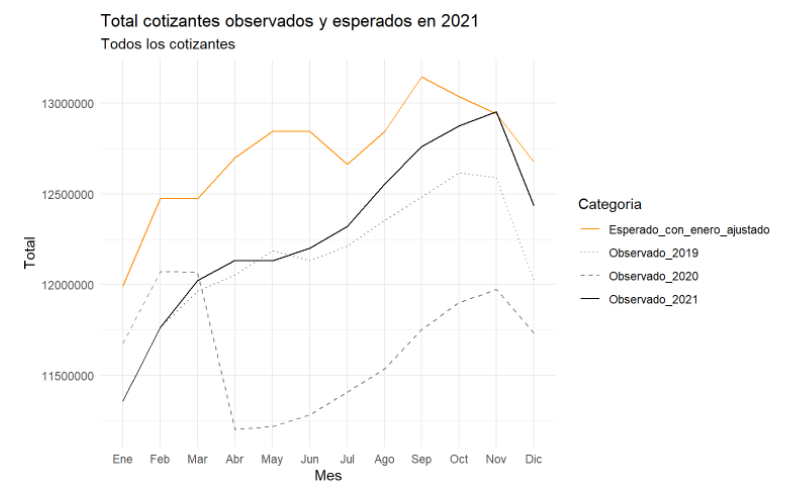
\includegraphics[width = 12.5cm]{figures/01_dinamica/serie_contraste.png}
\caption{Comparativo anual de las cotizaciones}
\label{figura:IEM_Total}
\end{wrapfigure}

El resultado presentado en la figura \ref{figura:IEM_Total} muestra el comportamiento del total de cotizantes para 2019, 2020 y 2021. Se puede observar que para el mes de diciembre hay un decrecimiento esperado atribuido al comportamiento estacional del número de cotizantes. Este comportamiento ocurre tanto para cotizantes dependientes como independientes. (\href{https://www.ugpp.gov.co/Evolucion-cotizaciones-Sistema-Proteccion-Social}{Ver presentación - Dic21}). 


\textcolor{red}{
El número de cotizantes es de \textbf{12.434.346} (5.9\% más que en diciembre de 2020). En términos interanuales, los cotizantes dependientes se observó un crecimiento del 7.2\%. De este grupo de cotización se pudo establecer que el mayor crecimiento se da en el grupo de cotización de Hasta 1 SMMLV (10.8\%), mientras que aquellos entre 1 y hasta 2 SMMLV presentaron el menor crecimiento con 6.3 \%. Por otro el número de cotizantes independientes creció un 0.8\%. Siendo los cotizantes de hasta 1 SMMLV los que presentaron un crecimiento mayor (16.5\%). Para este mismo grupo de cotización se encontró un crecimiento negativo -2.1\% par el grupo de 1 SMMLV. 
En términos de el comportamiento del último semestre, se puede ver que para los cotizantes dependientes existe un decrecimiento el número de cotizantes para los meses de noviembre y diciembre en los grupos de 1 SMMLV (-1.8\% y -17.9\%) y, entre 2 y hasta 5 SMMLV (-3.9\% y -0.6\%). }


\FloatBarrier

\subsection{Resumen Cotizaciones}

El número de cotizantes total a diciembre de 2021 es de \textbf{12.434.346} (5.9\% más que en diciembre de 2020). En términos interanuales, para los cotizantes dependientes se observó un crecimiento del 7.2\%. De este grupo se pudo establecer que el mayor crecimiento se da para aquellos que se encuentran en el rango de IBC menor que un SMMLV (10.8\%), mientras que aquellos que cotizan un SMMLV presentaron el menor crecimiento con 5.6 \%, aunque para este conjunto, en términos de la variación mensual para el último semestre, se observa un decrecimiento en los meses de noviembre y diciembre (-1.8\% y -17.9\% respectivamente). Por otro lado, el grupo de cotizantes dependientes con IBC mayor a 5 SMMLV tuvo un aumento considerable entre los meses de noviembre y diciembre (7.6\%), el cual es sostenido a partir del crecimiento que se presentó entre octubre y noviembre (20.5\%). Dicho cambio se ve reflejado en el aumento de 71.173 cotizantes en el comportamiento interanual.

En el caso del grupo de independientes, la cantidad de cotizantes creció un 0.8\% con respecto a diciembre del año anterior, siendo los cotizantes con IBC menor a un SMMLV los que presentaron el crecimiento mayor (16.5\%). En contraste, el conjunto de cotizantes independientes de un SMMLV presentó un decrecimiento de 2.1\%. Para diciembre, el número de cotizantes independientes disminuyó con respecto al mismo periodo del año anterior, aunque el crecimiento mensual para aquellos con IBC menos a un SMMLV fue de 26.3\%.

\begin{table}[!h]
\centering
\begin{minipage}{0.5\textwidth}
  \centering
  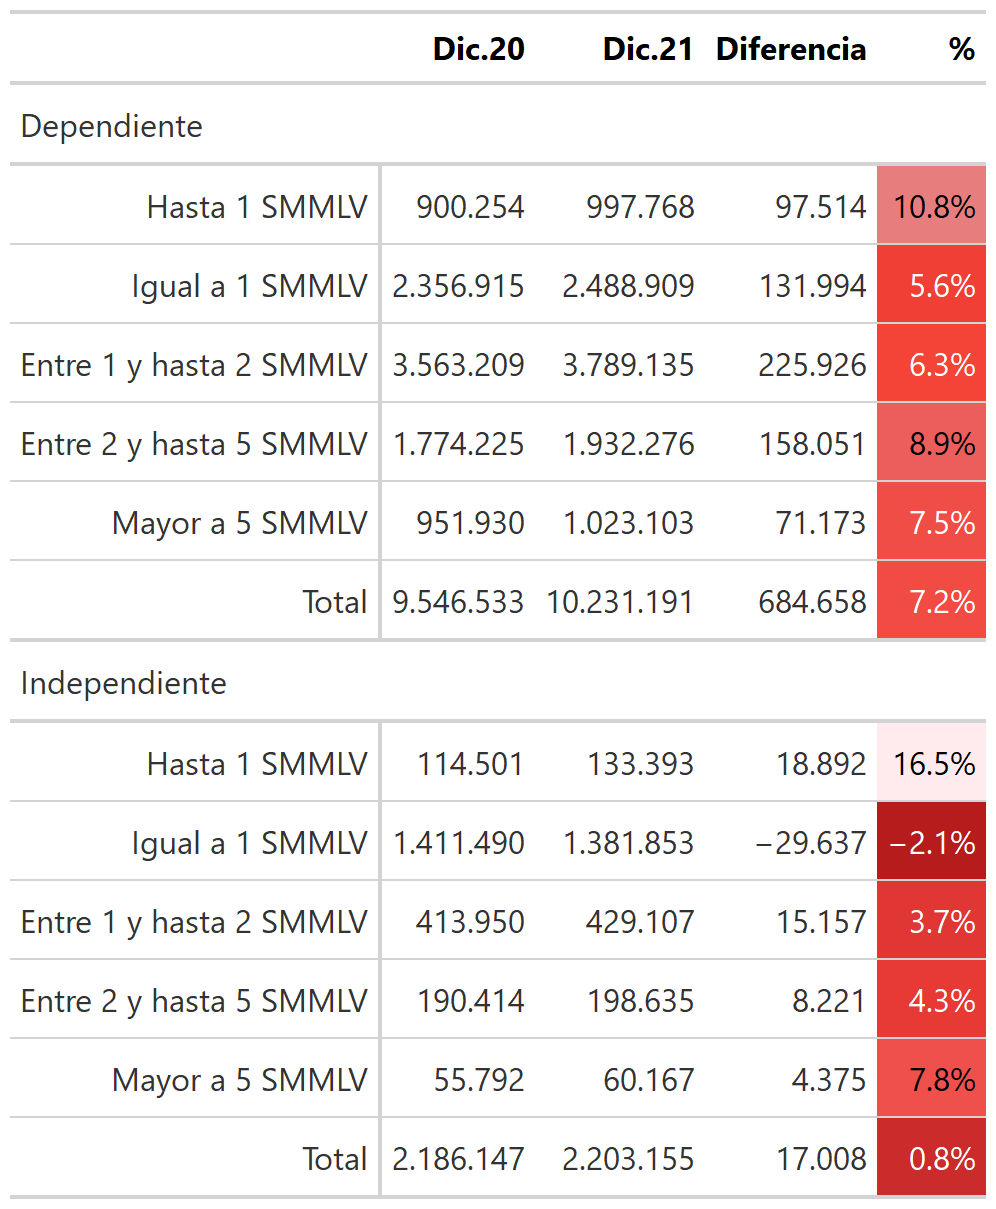
\includegraphics[width=0.6\linewidth]{results/01_dinamica/salida_total_cotizantes.png}
\end{minipage}%
\begin{minipage}{0.5\textwidth}
  \centering
  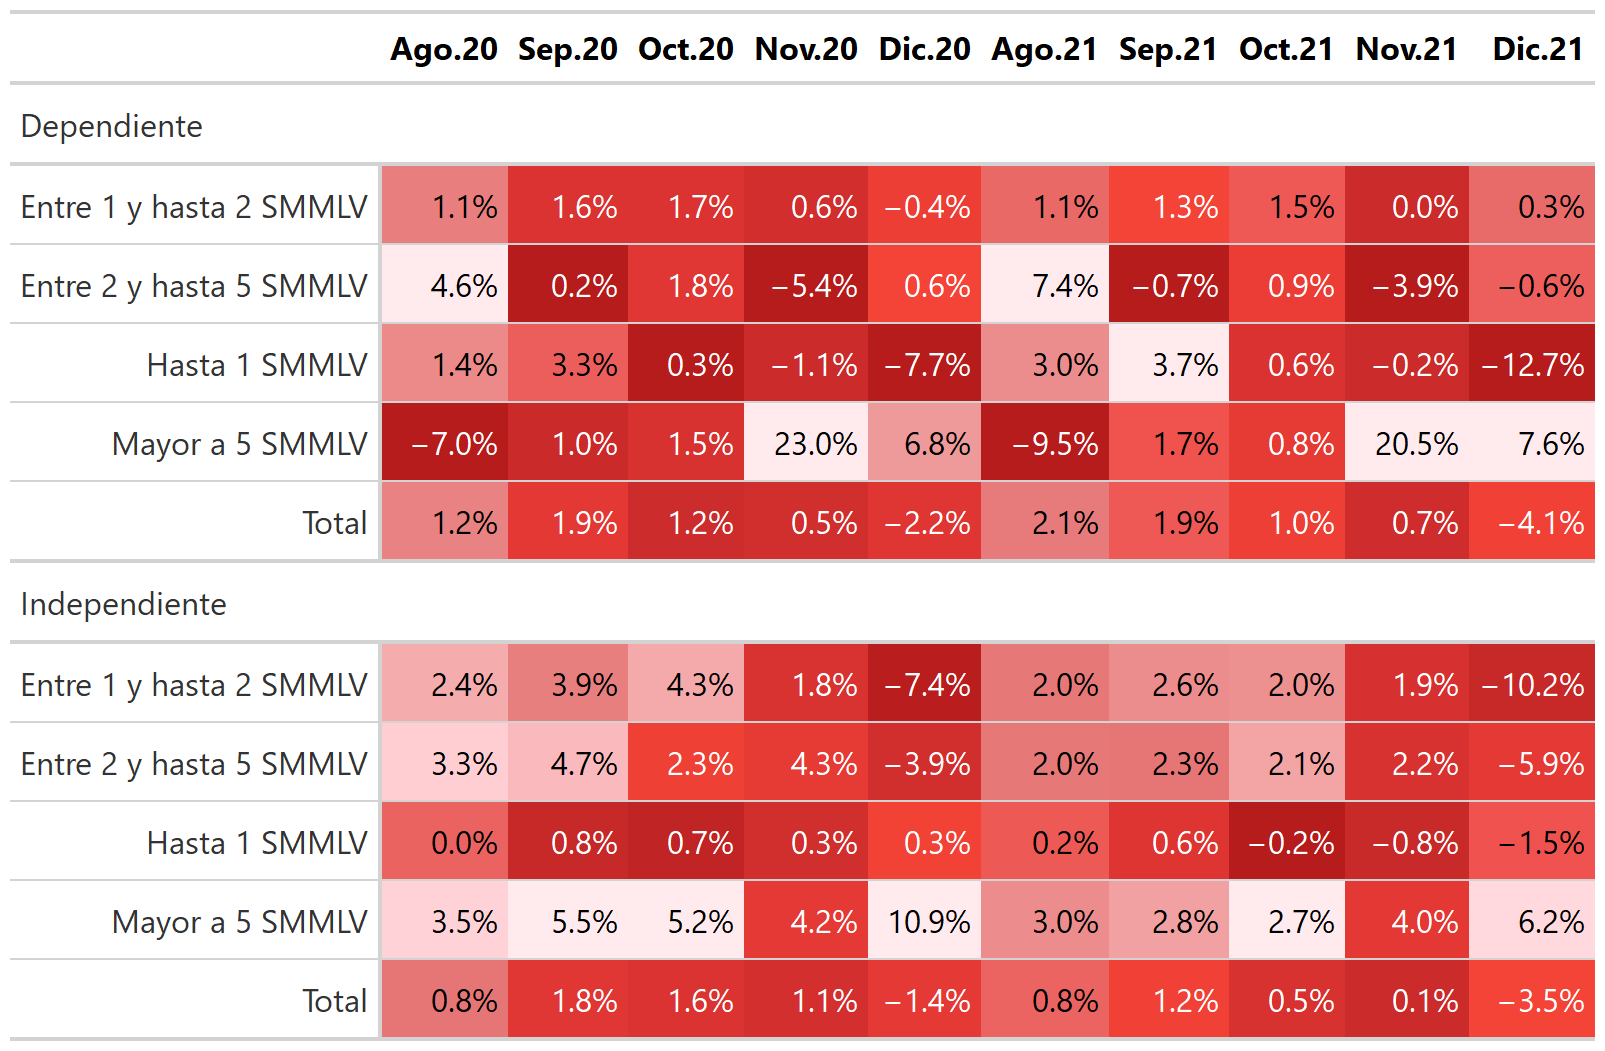
\includegraphics[width=\linewidth]{results/01_dinamica/salida_total_cotizantes_variaciones.png}
\end{minipage}
\caption{
Resumen número de cotizantes por rango salarial (IBC). Totales y variación anual (Izq.), variaciones mensuales (Der.)
}

\label{tabla:resumen:cotizantes_rangoIBC}
\end{table}

\vspace{0.5cm}
\subsection{Novedades}
\begin{wrapfigure}{r}{0pt}
\raisebox{0pt}[\dimexpr\height-1.6\baselineskip\relax]{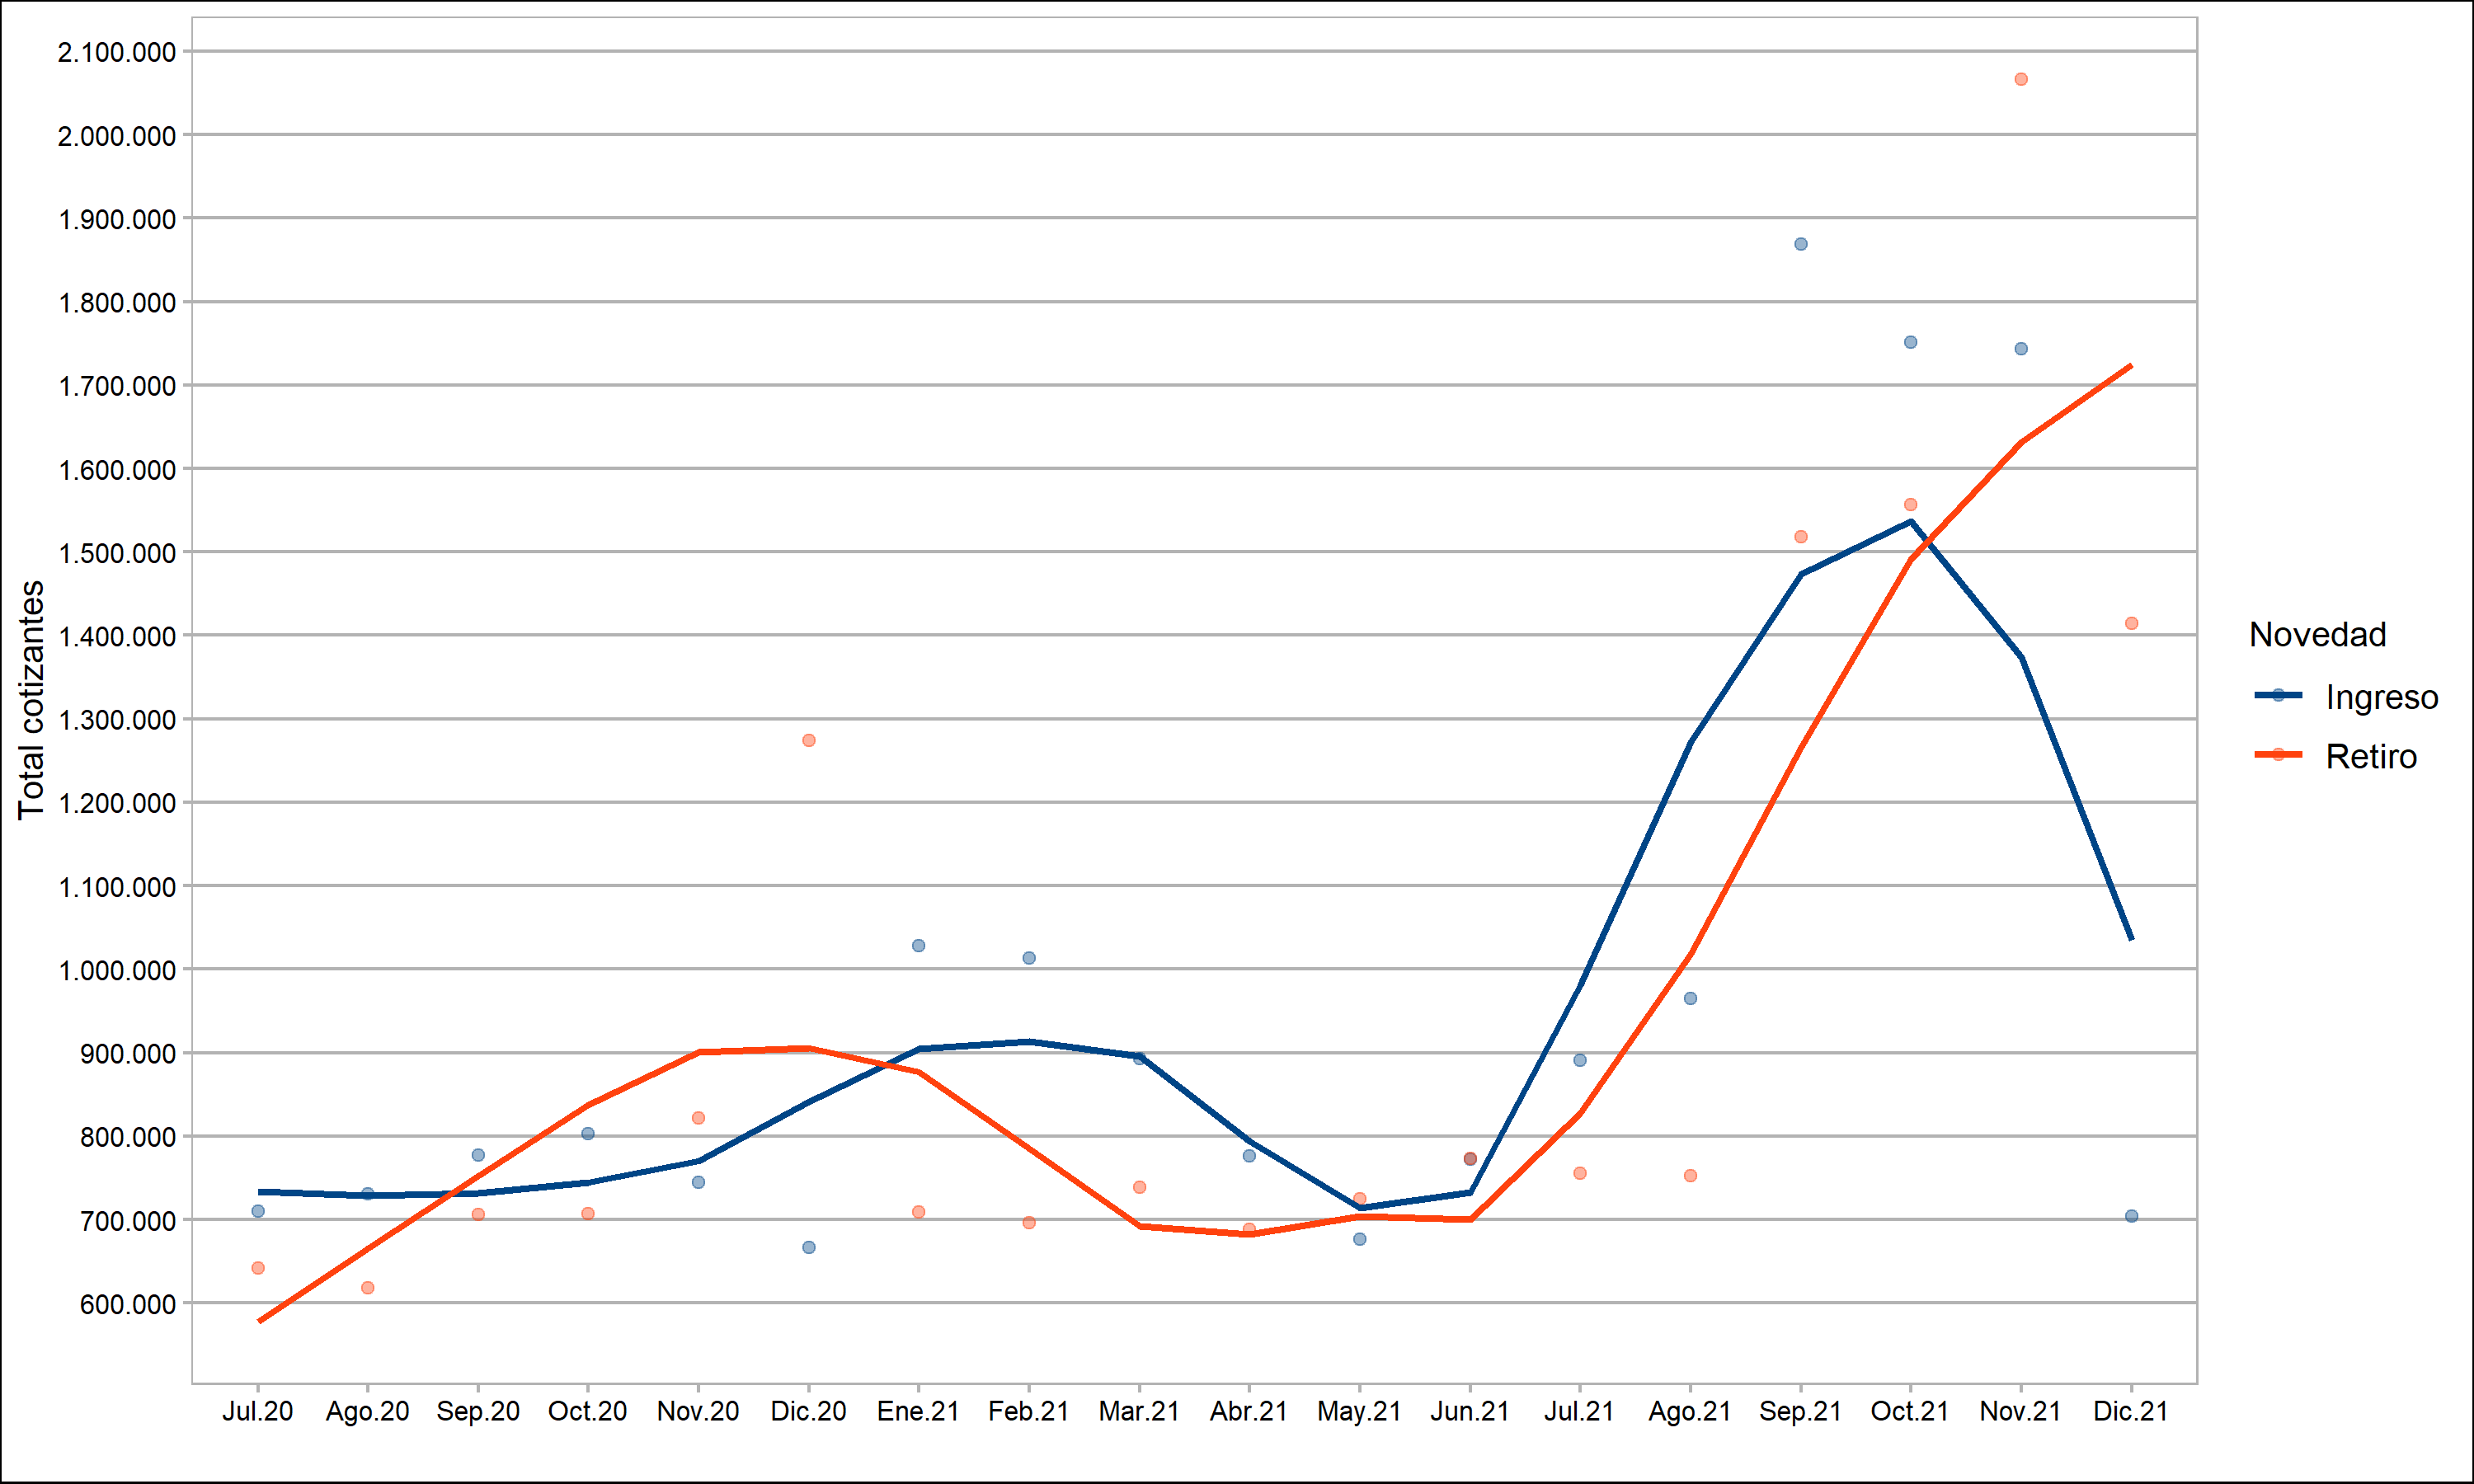
\includegraphics[width = 11.5cm]{figures/01_dinamica/total_novedades_dependientes_ingret.png}}
\caption{Comparación del total de novedades para dependientes (ingresos, retiros)}
\label{figura:novedad:sectorprivado:IR}
\end{wrapfigure}

Las novedades tienen cinco categorías de interés: ingresos, retiros, suspensiones, incapacidades y vacaciones. Las novedades de ingresos y retiros se analizan a través de las Figuras \ref{figura:novedad:sectorprivado:IR} y \ref{figura:novedad:indpependientes:IR} en las que se puede evidenciar la evolución de las cifras en los últimos 18 meses. Para las novedades por suspensiones, incapacidades y vacaciones se presenta un comparativo interanual acompañado de una evolución anual de los cotizantes dependientes (Cuadro \ref{tabla:novedades:dependientes}). 


Para los cotizantes dependientes se observa que los ingresos son menores a los retiros representando un cambio neto de \textbf{710.423} cotizantes para diciembre 2021. Se encuentra que para el año 2020 la diferencia neta es de 607.152. Sin embargo, la diferencia anual en el número de retiros es de 140.383, mientras que los ingresos tienen una diferencia de 37.112. Las tendencias a lo largo de los 18 meses muestran un comportamiento estacional tanto en ingresos como en retiros para los últimos meses del año, donde la cantidad de novedades crece. A pesar de dicha similitud de tipo cíclico, se puede ver que a partir de junio de 2021 dónde, retiros e ingresos tienen totales similares, el incremento en ambas condiciones es notable. Se pudo determinar que a partir de agosto 2021 el incremento en el número de retiros de No-Privados pasó de 88.362 a 203.583, y para dependientes privados de 666.497 a 1.210.871. 


La dinámica de las suspensiones, incapacidades y vacaciones han tenido un cambio sustancial a lo largo del comparativo anual (Ver Cuadro \ref{tabla:novedades:dependientes}).Las suspensiones aumentaron en 50.668 en el comparativo de Diciembre 2020 y 2021. Tanto las novedades por incapacidades como vacaciones tienen un aumento en el mes de diciembre, 1.8\% y 16.1\% respectivamente. Los gráficos de tendencias muestran que para 2020 se presentaron una mayor cantidad de suspensiones al comenzar el ano producto de la pandemia por COVID-19. De otro lado para 2021, las suspensiones tienen valores bajos en los primeros meses del año, mientras que en los meses de octubre, noviembre y Diciembre aumentan considerablemente. El comparativo para las vacaciones muestra para el 2021 que el máximo se encuentra en diciembre, el cual difiere del comportamiento para 2020 el cual corresponde una vez más al impacto de la pandemia en el comportamiento del SPS.


\begin{table}[!h]
\centering
\begin{minipage}{0.5\textwidth}
  \centering
  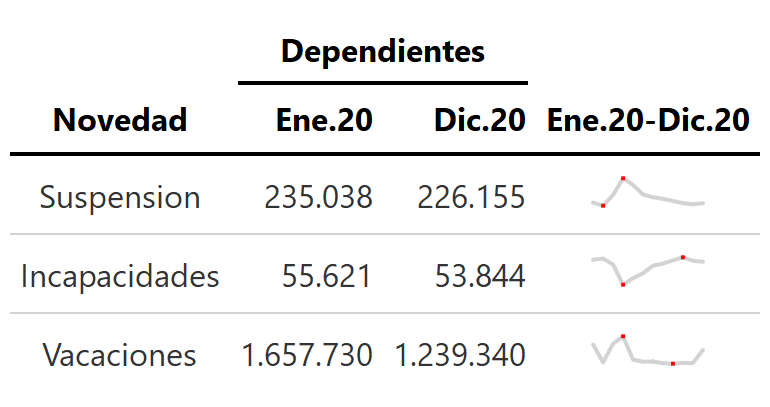
\includegraphics[width=\linewidth]{results/01_dinamica/salida_dependientes_novedades_resto_comparativo.png}
\end{minipage}%
\begin{minipage}{0.5\textwidth}
  \centering
  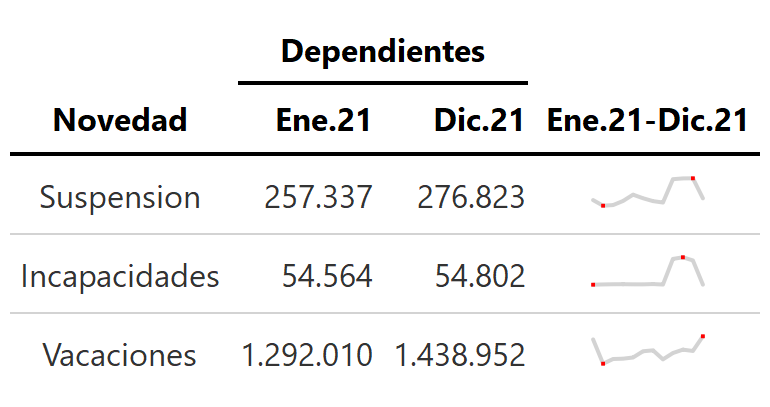
\includegraphics[width=\linewidth]{results/01_dinamica/salida_dependientes_novedades_resto.png}
\end{minipage}
\caption{Total novedades y tendencia anual}
\label{tabla:novedades:dependientes}
\end{table}

\begin{wrapfigure}{l}{0.6\textwidth}
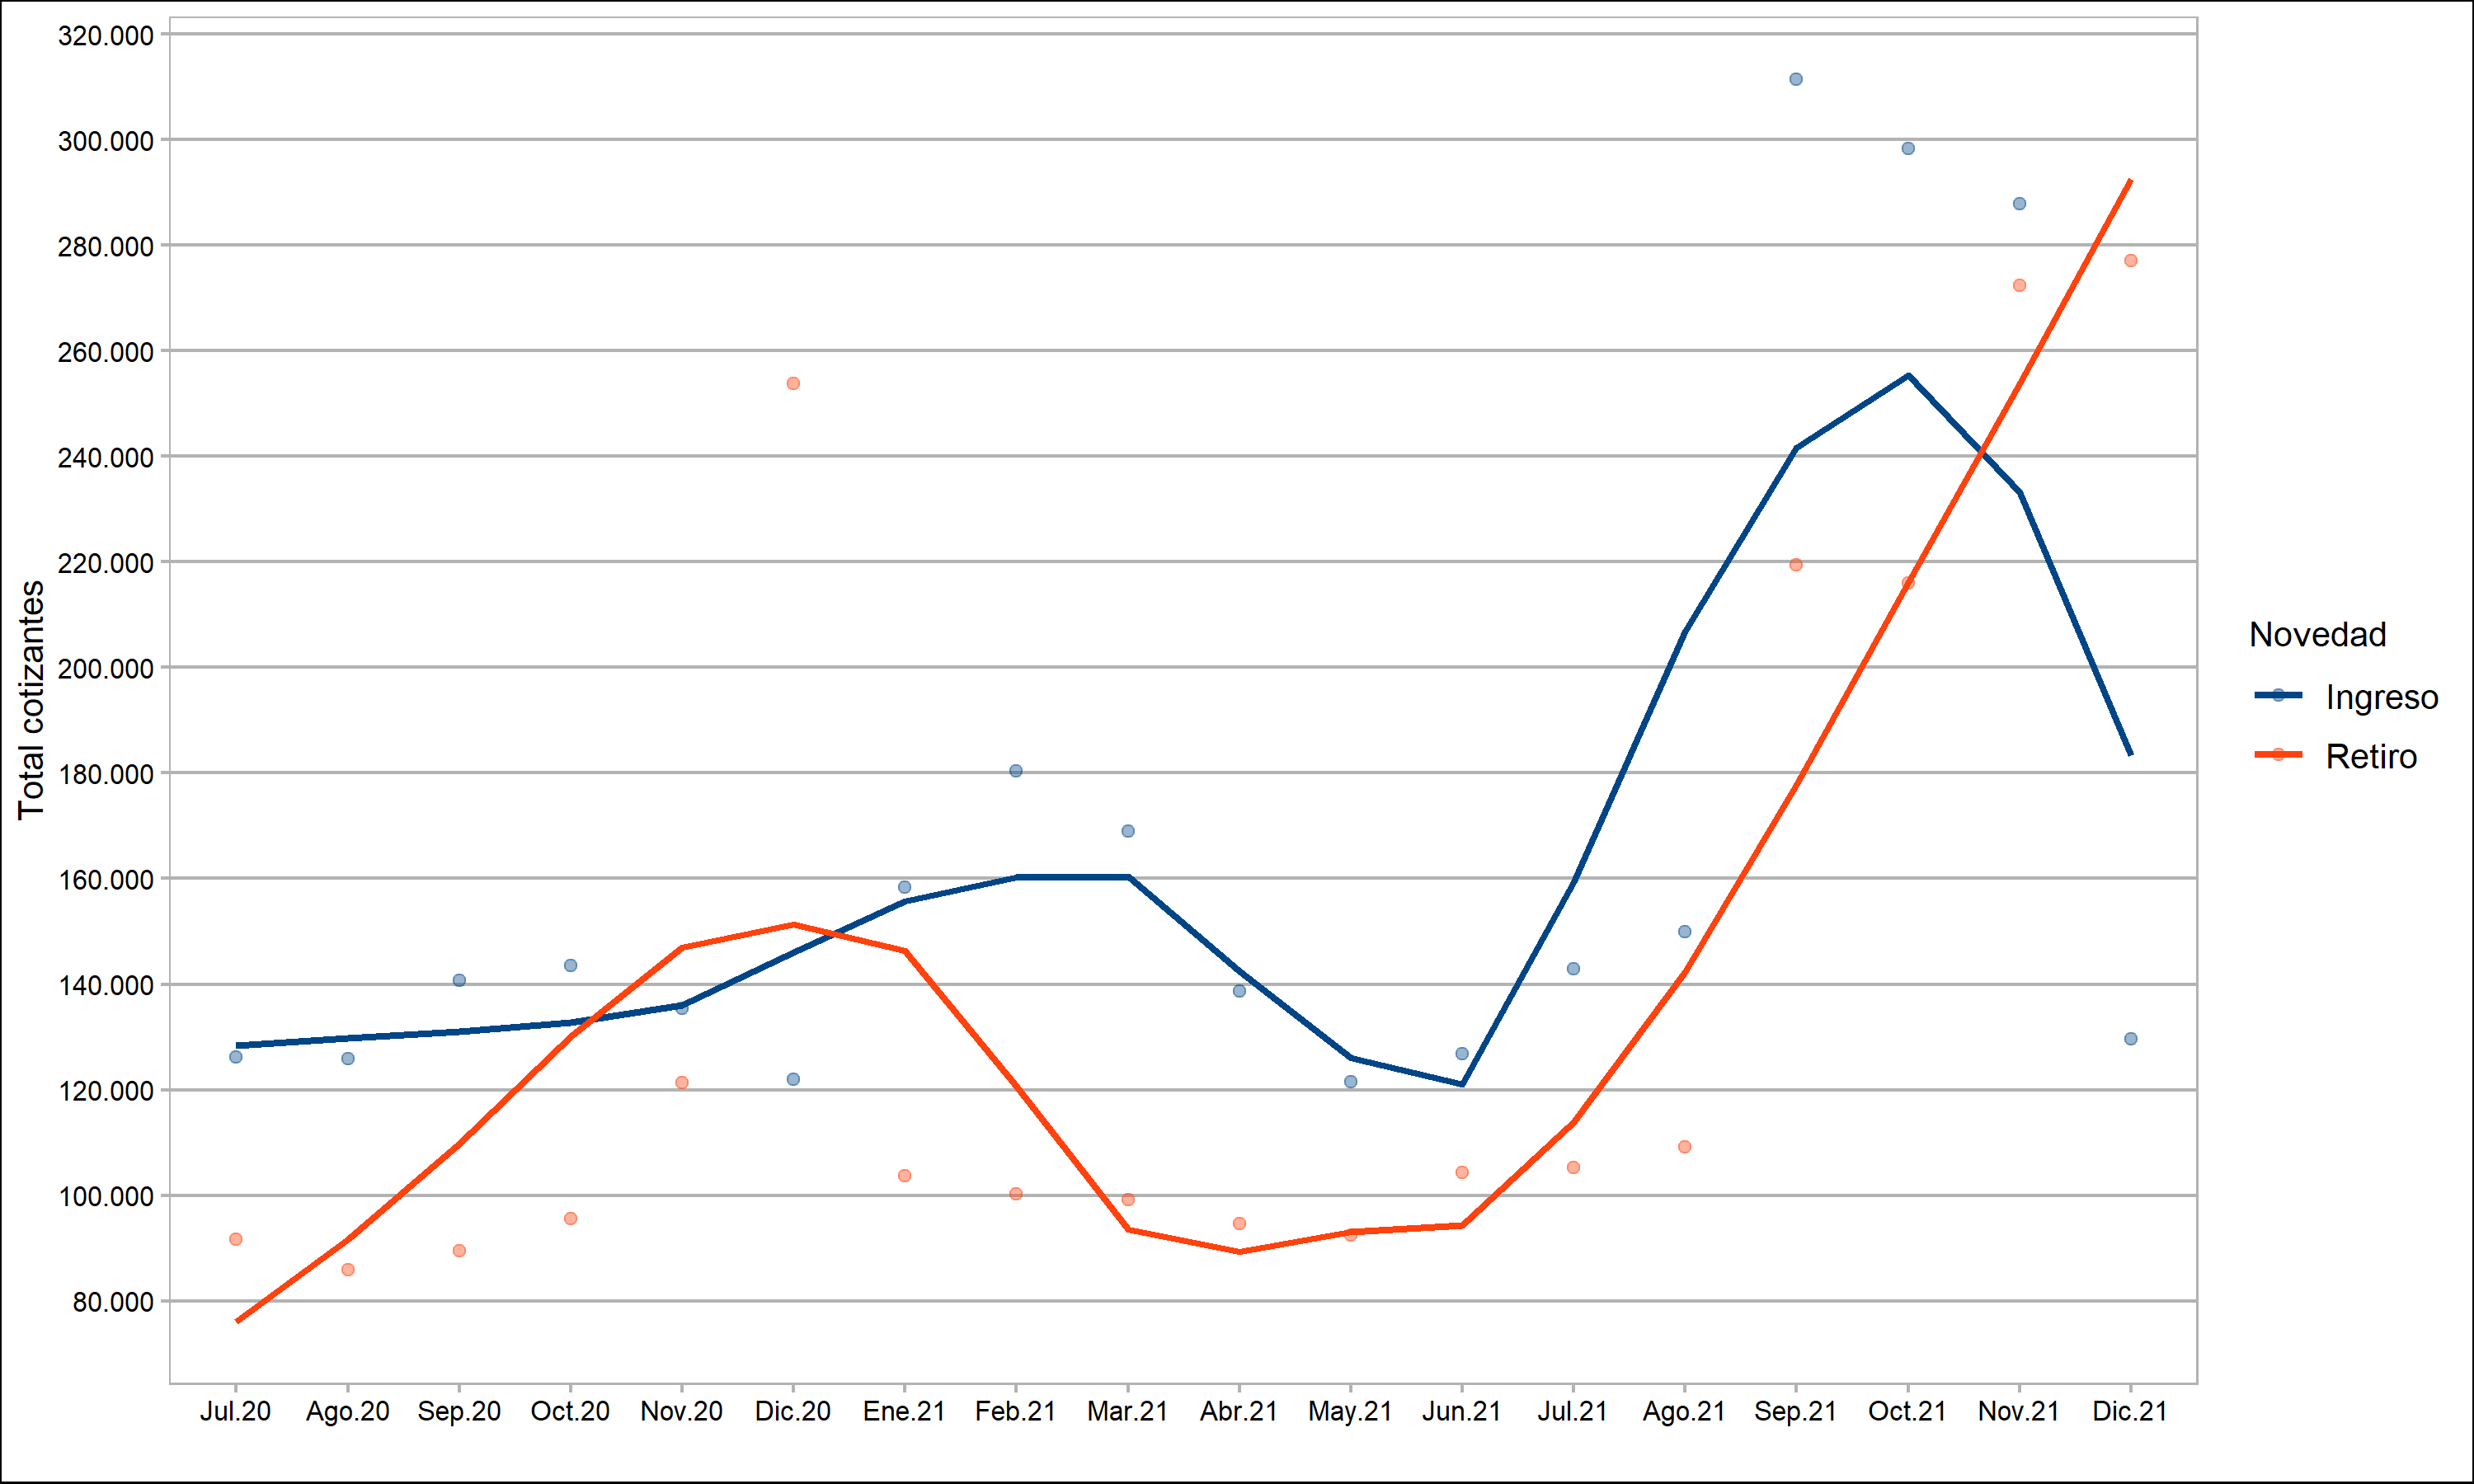
\includegraphics[width = 11.5cm]{figures/01_dinamica/total_novedades_independientes_ingret.png}
\caption{Comparación del total de novedades para independientes}
\label{figura:novedad:indpependientes:IR}
\end{wrapfigure}

La dinámica de las suspensiones, incapacidades y vacaciones han tenido un cambio sustancial a lo largo del comparativo anual (Ver Cuadro \ref{tabla:novedades:dependientes}). Las suspensiones aumentaron en 50.668 en el comparativo de diciembre 2020 y 2021. Tanto las novedades por incapacidades como vacaciones tienen un aumento en el mes de diciembre, 1.8\% y 16.1\% respectivamente. Los gráficos de tendencias muestran que para 2020 se presentó una mayor cantidad de suspensiones al comenzar el año producto de la pandemia por COVID-19. De otro lado para 2021, las suspensiones tienen valores bajos en los primeros meses del año, mientras que en los meses de octubre, noviembre y diciembre aumentan considerablemente. El comparativo para las vacaciones muestra para el 2021 que el máximo se encuentra en diciembre, el cual difiere del comportamiento para 2020 el cual corresponde una vez más al impacto de la pandemia en el comportamiento del SPS.



